\documentclass[aspectratio=1610]{beamer}
\usepackage{hyperref}
\usepackage[T1]{fontenc}

% other packages
\usepackage{latexsym,amsmath,xcolor,multicol,booktabs,calligra}
\usepackage{graphicx,pstricks,listings,stackengine}
\usepackage{ragged2e}
\usepackage[backend=bibtex,sorting=none]{biblatex} % biblatex
\setbeamerfont{footnote}{size=\tiny}
\addbibresource{ref.bib}

\usepackage{lipsum}

\author{Zhouxin Xue, Xuanhang Diao}
\title{Scheduling Beyond CPUs for HPC}
\subtitle{Fan Y, Lan Z, Rich P, et al. \\
\textit{HPDC 19} 
}

\institute{
    School of Biomedical Engineering, \\
    ShanghaiTech University \\
}
\date{14, April}
\usepackage{shanghaitech}

% defs
\def\cmd#1{\texttt{\color{red}\footnotesize $\backslash$#1}}
\def\env#1{\texttt{\color{blue}\footnotesize #1}}
\definecolor{deepblue}{rgb}{0,0,0.5}
\definecolor{deepred}{rgb}{0.6,0,0}
\definecolor{deepgreen}{rgb}{0,0.5,0}
\definecolor{halfgray}{gray}{0.55}

\lstset{
    basicstyle=\ttfamily\small,
    keywordstyle=\bfseries\color{deepblue},
    emphstyle=\ttfamily\color{deepred},    % Custom highlighting style
    stringstyle=\color{deepgreen},
    numbers=left,
    numberstyle=\small\color{halfgray},
    rulesepcolor=\color{red!20!green!20!blue!20},
    frame=shadowbox,
}

\begin{document}

\begin{frame}
    \titlepage
    \begin{figure}[htpb]
        \begin{center}
            
\includegraphics[keepaspectratio, scale=0.2]{pic/ShanghaiTech_Logo.png}
        \end{center}
    \end{figure}
\end{frame}

\section{Background Knowledge}

\begin{frame}{Pareto set}
    A \textbf{Pareto set} is a set of optimal solutions, where no objective can be improved without worsening another objective.
\end{frame}

\begin{frame}{Burst Buffer}
    A \textbf{Burst Buffer} is an intermediate storage layer positioned between compute nodes and parallel file systems (PFS) in high-performance computing (HPC) systems. 
    \begin{itemize}
        \item Absorb the bursty I/O data generated by data-intensive applications.
        \item Built from solid-state drives (SSDs).
        \item Can be either attached to compute nodes as local resources or configured as global resources shared by compute nodes.
    \end{itemize}
\end{frame}

\section{Background and Motivation}

\begin{frame}{Multi-Resource Scheduling}

    \begin{itemize}
        \item HPC systems are equipped with diverse global and local resources.
        \item HPC job scheduler plays a crucial role in efficient use of resources.
    \end{itemize}

    \begin{figure}[htpb]
        \begin{center}
            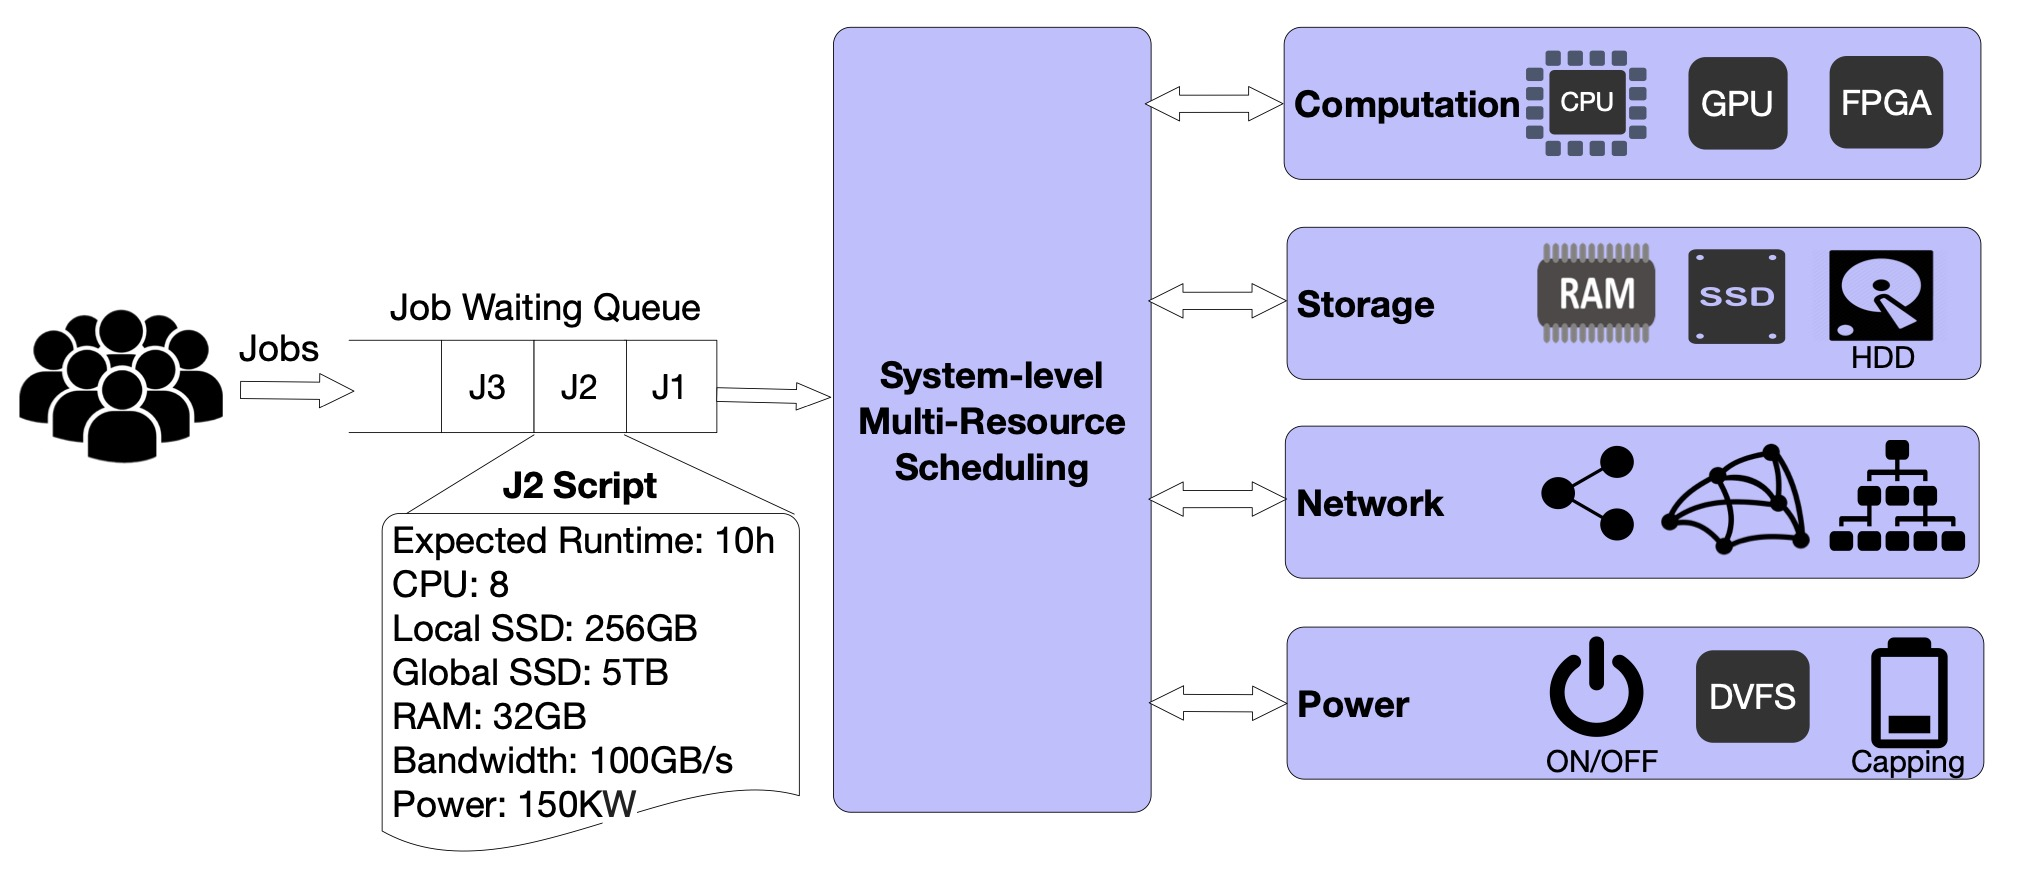
\includegraphics[keepaspectratio, scale=0.12]{pic/sched_with_multi_res.jpeg}
        \end{center}
        \caption{HPC job scheduling problem involves in multiple resources.}
        \label{fig:sched_with_multi_res}
    \end{figure}
   
\end{frame}

\begin{frame}{Limitations of Existing Scheduling Methods}
    
    Existing methods often overlook alternative solutions or optimal resource combinations, leading to under-utilization of resources or poor application performance.
    
    \begin{itemize}
        \item Naive method
        \item Constrained method
        \item Weighted method
        \item Bin packing method
    \end{itemize}
    
\end{frame}

\begin{frame}{Goal}

    The Motivation of the this paper is to improve overall resource utilization and reduce job wait time in HPC systems.

    \begin{itemize}
        \item providing rapid scheduling decisions
        \item minimizing the impact on site policies
        \item ensuring extensibility to accommodate emerging resources
    \end{itemize}
   
\end{frame}

\section{Methodology of BBSched}

\begin{frame}{}
    
\end{frame}


\end{document}